\subsection{Preprocessing techniques}
In this section, we consider the attack information as noise in the image. We assume attackers tend to control the magnitude of their attacks so as not to be detected by the system, but make them effective enough to misguide the system to the wrong results. We then make use of this effect, and consider the problem from the image preprocessing perspective. We use different approaches, rescaling, bit-depth reduction and total variation, to remove the attack or adversarial perturbations in the input data before we fit into the net, and also try to maintain enough information for our net to give the right results.

\subsubsection{Bit-Depth Reduction} %reference needed here
Bit-Depth reduction approach is to reduce the color depth in bits. We know that each RGB channel has 8-bits, which is possible to be reduced. We then consider removing the noise by reducing the original 8-bit images to fewer bits, as a try to remove the adversarial attack but not significantly destroying the recognisability of the images. 

Before we introduce the way doing bit-depth reduction, we notice that our input values are in the range [0,1]. Then more specifically, for reducing from 8 bits to i bits, we first multiply the input data by ($2^i - 1$),then round to zeros, and scale the values back to the the range [0,1]. Hence we successfully reduce the information capacity from the original 8-bit to i-bit with the critical step of integer rounding. 




\begin{figure}[h!]
	\centering
	\begin{subfigure}{.35\textwidth}
		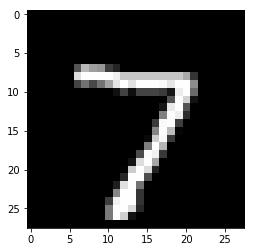
\includegraphics[width=\textwidth]{original7.png}
		\caption{Original image}
		\label{fig: bit-depth reduction 1}
	\end{subfigure}
	\begin{subfigure}{.35\textwidth}
		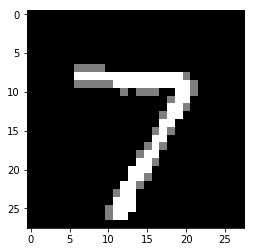
\includegraphics[width=\textwidth]{bit1-7.png}
		\caption{bit-one image}
		\label{fig: bit-depth reduction 8}
	\end{subfigure}
	\caption{Bit-depth reduction image}
\end{figure}

We can see for MNIST database, even we reduce the color depth to just 1 bit, it is very clear and does not introduce human-observable loss. But for images in colored ImageNet, it do shows significant loss when we reduce the bit-depth to be less than 4, which can also be inferred from the decrease in the accuracy in the following results section. 


\subsubsection{Median, LAP and LAR Smoothing Filters}
It has been shown that by implementing median filtering, local average with neighbourhood pixels (LAP) and the local average with radius (LAR) pre-processing noise filters on the input image data it is possible to effectively reverse the mis-classifications caused by adversarial perturbations and significantly decrease the efficiency of the attack \cite{khalid2019fademl}. 

\begin{figure}[h!]
	\centering
		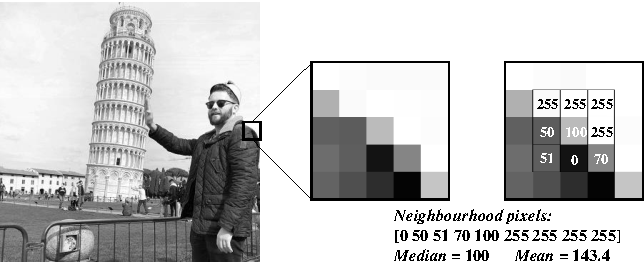
\includegraphics[width=.72\textwidth]{Diagram1-cropped.pdf}
		\caption{Original image}
		\label{fig: Median}
	\caption{Median filtering to remove impulse (or salt-and-pepper) noise}
\end{figure}



\begin{figure}[h!]
	\centering
	\begin{subfigure}{.3\textwidth}
		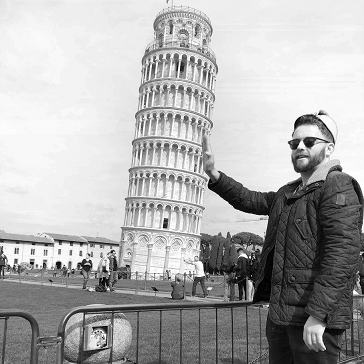
\includegraphics[width=\textwidth]{Iorig.png}
		\caption{Original image}
		\label{fig: LAPLAR1}
	\end{subfigure}
	\begin{subfigure}{.3\textwidth}
		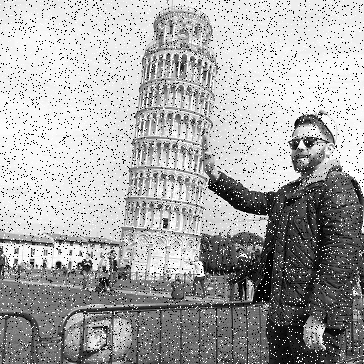
\includegraphics[width=\textwidth]{Inoise.png}
		\caption{Impulse noise inserted}
		\label{fig: LAPLAR2}
	\end{subfigure}
	\begin{subfigure}{.3\textwidth}
		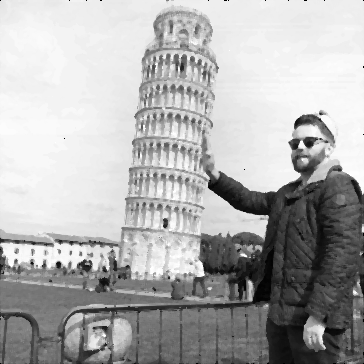
\includegraphics[width=\textwidth]{Ifiltered.png}
		\caption{Median filtering noise}
		\label{fig: LAPLAR3}
	\end{subfigure}
	\caption{Median filtering to remove impulse (or salt-and-pepper) noise}
\end{figure}
These standard noise filtering algorithms are easy to implement and can significantly retrieve correct classification confidence lost to the perturbations, whilst maintaining the visual structure of the image. Other similar forms of pre-processing include JPEG compression (lossy image compression) where the image is irreversibly encoded so as to reduce the file size, and image quilting where 



\subsubsection{Total Variance Minimisation}

\subsubsection{Defence GAN}
In considering solutions to the pre-processing defence to adversarial attacks, in particular FGSM, we note that all our proposed methods are attempting in some way to smooth out the noise in a poisoned image and classify the result. An alternative is to ask can we classify a different image with the same semantic content as the poisoned image but without the poison.  This method suggests we could use a generative model of our dataset to generate in domain data which would remove any chance of classifying a poisoned image.  The remaining question is how to condition the generator to create images with the same semantic content of the poisoned image without introducing the poison to our approach?

This idea has been recently introduced by [TODO citation] where they report good success in defending againsts adversarial attacks.

